\section{第2問：LLMの心の理論を最小対で調べる}
\subsection{問いと検証方針}
心の理論（Theory of Mind; ToM）は、他者の知識・信念・意図が自分や現実と異なる場合も、それを表現して行動を予測する能力である。
LLMが文章問題に正答することはToMに整合する行動的証拠になるが、主観的な心を持つことの直接証拠にはならない。
そこで本実験では、「現実の状態だけを答える」「登場人物は必ず間違う」「褒め言葉は常に褒めている」といった単純な規則から区別できるかを調べた。

先行研究では、誤信念問題に真信念対照を加え、表面的な解き方を排除する方法が用いられている\cite{kosinski}。
また、失言の理解は質問形式や断定の慎重さの影響を受けることが報告されている\cite{strachan}。
本実験も情報アクセスを変えた対照と、情報不足なら断定しない問題を加える。
有名な人名や容器の物語をそのまま引用せず、撮影・実験・合奏・展示会など独自の場面を作った。

\subsection{36項目の構成と取得手順}
一次信念、二次信念、皮肉、失言における知識帰属を各8項目、情報不足の対照を4項目作った。
前4群はそれぞれ4組の最小対であり、対の両方が正解した場合のみその組を成功とする厳格な指標も計算した。
例えば一次信念では、綾がレンズを赤いケースに入れた後、航が青いロッカーへ移す。
「通知が来たが端末の電源が切れていて未読」と「移動の映像を最後まで見た」を入れ替える。
レンズの実在場所は同じでも、綾が最初に探す場所の予測は変わる。

\begin{figure}[tb]\centering
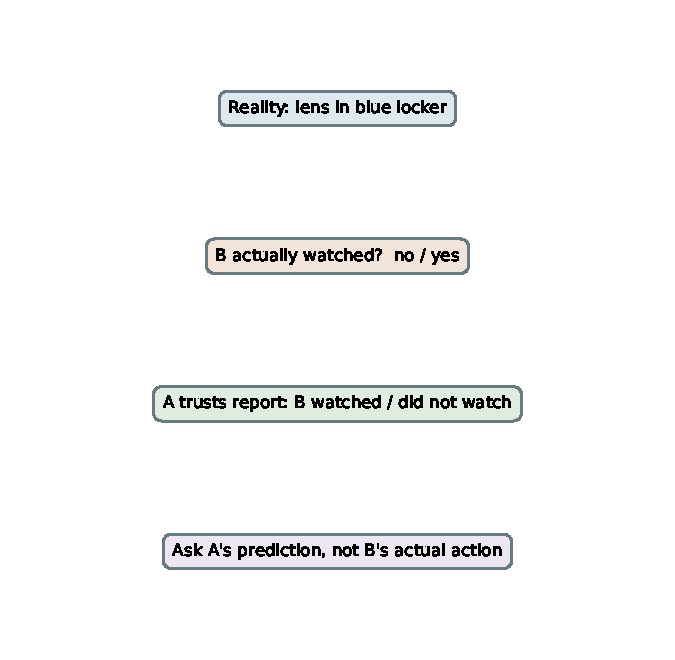
\includegraphics[width=\linewidth]{02/results/belief_intervention.pdf}
\caption{現実を固定して情報アクセスに介入する最小対。登場人物の信念と解答者が知っている現実を分離する。}
\end{figure}

二次信念では、綾が航の画面故障を知る条件と、航の映像視聴を確認した条件を比較し、綾による航の探索場所の予測を問う。
皮肉では、同じ肯定表現に対して、仕事の失敗と成功という文脈を変えた。
失言では、作者の目の前で作品を批判した発言者について、作者を知らなかった場合と知っていた場合を区別した。
どちらも相手は傷つきうるので、「失礼かどうか」と「無知による失言かどうか」を同一視しない。
情報不足群では、褒め言葉しか残っていないメッセージから、皮肉か称賛かを確定できるかを問う。
選択肢A/B/Cは項目ごとに巡回置換し、正答文字の偏りを抑えた。

作成後のプロンプトJSONを固定し、異なる二つの新規コンテキストのCodexサブエージェントに、正解ファイルと相互の回答を見せずに回答させた。
各コンテキストへ36項目を一括で渡し、選択肢と短い根拠を保存した。
モデルは\texttt{gpt-6.1-sol}、実施日は2026年11月17日である。
温度など内部の生成設定は取得できないため、温度0のAPI実験とは記載しない。
1コンテキスト内では項目が同時に見えるので、36項目がそれぞれ完全に独立した会話であるわけでもない。
元データ、生回答、正解、採点コード、SHA-256ハッシュを保存した。

\subsection{実測結果と対照}
両コンテキストとも36/36項目を正答し、16組全ての最小対にも成功した。
コンテキスト間の選択肢一致は36/36であった。
常にAを選ぶ対照は12/36、信念問題で常に現実の最終場所を答える対照は8/16である。
後者との差は、単に最新の位置情報を答えたわけではないことを示す。
ただし、作成した有限の問題集合における観察であり、独立した72人分のデータとして検定することはしない。

\begin{figure}[tb]\centering
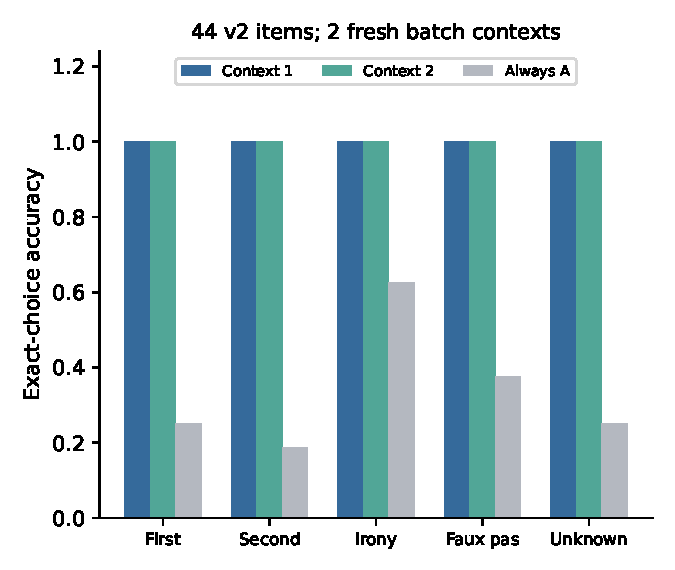
\includegraphics[width=\linewidth]{02/results/accuracy.pdf}
\caption{二つの新規コンテキストと固定回答対照の正答率。一次〜失言は各8項目、情報不足は4項目。高得点はこの問題集合での天井効果でもある。}
\end{figure}

一次信念の未読条件に対し、文脈1は「綾は移動の通知を読んでいないので、自分が入れた赤いケースにまだあると考えるから。」と説明し、古い場所を選んだ。
二次信念でも、対象者自身の知識と、それを予測する人物の知識を追跡した。
情報不足群では、両コンテキストとも称賛・皮肉のどちらかに無理に決めず、情報不足を選んだ。
この結果は、今回の短い日本語物語で情報アクセスと信念を対応づけられたことを支持する。
全問正解になった以上、このテストでは能力の上限や誤りやすい境界を特定できなかった点も結果として重要である。

\begin{table}[tb]\centering\footnotesize
\caption{全項目の監査表。0/1は情報条件の違い。プロンプト全文と短い根拠は公開JSONに保存。}
\begin{tabular}{lrrr}\toprule
項目群 & 項目数 & 文脈1 & 文脈2\\\midrule
一次信念 & 8 & 8 & 8\\
二次信念 & 16 & 16 & 16\\
皮肉 & 8 & 8 & 8\\
失言の知識 & 8 & 8 & 8\\
情報不足 & 4 & 4 & 4\\
\midrule
最小対の両問正解 & 20組 & 20 & 20\\
\bottomrule\end{tabular}

\end{table}

\subsection{ヒトとの類似性・相違と研究すべきデータ}
ヒトとの類似性は、見ていない出来事を他者が知らないと扱うこと、同じ言葉の意味を状況に応じて解釈すること、情報不足を認めることである。
一方、人間は視線・声の調子・身体の動き・過去の対人関係からも判断する。
本実験のLLMは、実際の相手と接する代わりに、実験者が明示した文章を処理している。
人間の対照群を測定していないため、今回の100\%から人間以上と結論づけることはできない。
同じ形式を多数見たことによる規則適用と、他者の心の柔軟なモデル化のどちらが主なのかも、この結果だけでは決められない。

類推推論については、レンズ・センサー・鍵・基板という異なる対象の物語に、共通する「観察できた情報だけで信念を更新する」という関係を対応させられるかが焦点となる。
表面的な物の置換だけでなく、ソフトウェアのアクセス権、共同作業の共有履歴、誤った地図を用いる相手との協調などへ移したテストが望ましい。
類推の役割は仮説として有力でも、強いAIの十分条件が証明されたわけではない。

今後集めるべきデータは、各人物が各時点で何を見聞きしたかを注釈した時系列対話、情報を意図的に隠す協調課題、誤解の指摘後に信念を修正する長期的な対話である。
正解ラベルに加え、「まだ決められない」という不確実性、文化や関係性によって複数解が妥当になる場合の許容範囲も必要になる。
評価では、作成者とモデル系列を分け、未公開項目を独立に作り、言い換え・人物名・文順・不要情報の挿入への頑健性を検証すべきである。
今回の項目生成にも同系列のLLMを利用したため、出題側と被験側の独立性に限界がある。
公開後の同じテストによる将来モデルの評価には、学習データ混入の可能性も考慮する必要がある\cite{tomreview}。
\repolink{02}
